\documentclass[tikz,border=2pt]{standalone}
\renewcommand{\familydefault}{\sfdefault}
\usetikzlibrary{arrows.meta,calc,positioning}
\tikzset{every picture/.style={line width=1pt, >=Stealth},
         hl/.style={fill=black, fill opacity=0.12, text opacity=1}}
\begin{document}
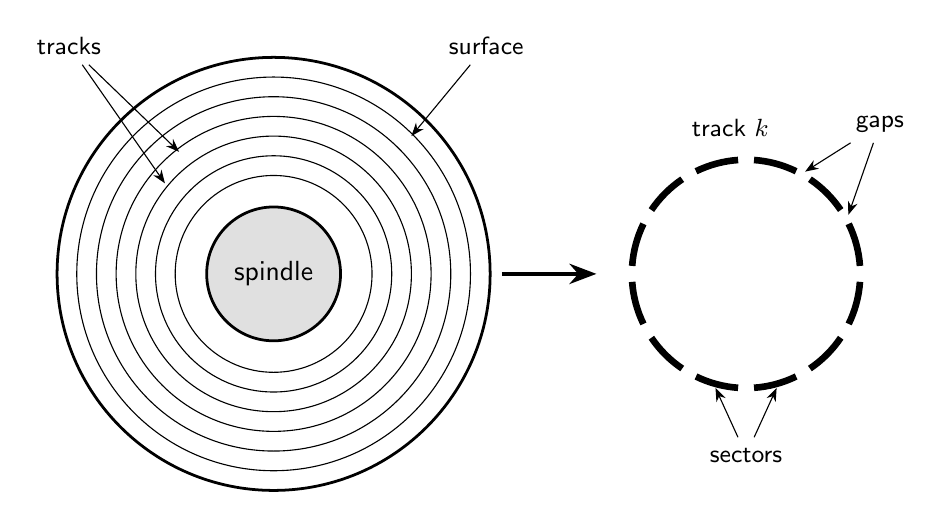
\begin{tikzpicture}[note/.style={font=\small}]
  % A surface holds concentric tracks around the spindle.
  \foreach \r in {1.25, 1.5, 1.75, 2, 2.25, 2.5} \draw[thin] (0, 0) circle (\r);
  \draw (0, 0) circle (2.75);
  \draw[hl] (0, 0) circle (0.85);
  \node at (0, 0) {spindle};
  \node[note] (surface) at (2.7, 2.9) {surface};
  \draw[->, thin] (surface) -- (1.75, 1.75);
  \node[note] (tracks) at (-2.6, 2.9) {tracks};
  \draw[->, thin] (tracks) -- (-1.2, 1.55);
  \draw[->, thin] (tracks) -- (-1.38, 1.15);
  \draw[->, line width=1.5pt] (2.9, 0) -- (4.1, 0);
  % One track is divided into sectors separated by gaps.
  \foreach \a in {0, 30, ..., 330} \draw[line width=2.4pt] (6, 0) ++(\a + 4:1.45) arc[start angle=\a + 4, end angle=\a + 26, radius=1.45];
  \node[note] at (5.8, 1.85) {track $k$};
  \node[note] (gaps) at (7.7, 1.9) {gaps};
  \draw[->, thin] (gaps) -- ($(6, 0) + (60:1.5)$);
  \draw[->, thin] (gaps) -- ($(6, 0) + (30:1.5)$);
  \node[note] (sectors) at (6, -2.3) {sectors};
  \draw[->, thin] (sectors) -- ($(6, 0) + (-105:1.5)$);
  \draw[->, thin] (sectors) -- ($(6, 0) + (-75:1.5)$);
\end{tikzpicture}
\end{document}
